\documentclass[ebook,10pt,oneside,openany,final, french, a4paper]{memoir}

\usepackage{babel}
\usepackage[utf8]{inputenc}

\usepackage[final]
           {listings}     % code listings
\usepackage{relsize}      % provide relative font size changes
\usepackage{underscore}   % remove special status of '_' in ordinary text
\usepackage{verbatim}     % improved verbatim environment
\usepackage{parskip}      % handle non-indented paragraphs "properly"
\usepackage{array}        % new column definitions for tables
\usepackage[normalem]{ulem}
\usepackage{color}        % define colors for strikeouts and underlines
\usepackage{amsmath}      % additional math symbols
\usepackage{mathrsfs}     % mathscr font
\usepackage{microtype}
\usepackage{multicol}
\usepackage{xspace}
\usepackage{fixme}
\usepackage{lmodern}
\usepackage[T1]{fontenc}
\usepackage[pdftex,
            pdftitle={Retro},
            pdfsubject={},
            pdfcreator={Vincent CHAMBRIN},
            bookmarks=true,
            bookmarksnumbered=true,
            pdfpagelabels=true,
            pdfpagemode=UseOutlines,
            pdfstartview=FitH,
            linktocpage=true,
            colorlinks=true,
            linkcolor=blue,
            plainpages=false
           ]{hyperref}
\usepackage{memhfixc}     % fix interactions between hyperref and memoir
\usepackage{xstring}
\usepackage{caption}
\usepackage{subcaption}
\usepackage{wrapfig}
\usepackage{amsfonts}
\usepackage{stmaryrd}
\usepackage{cite}
\usepackage{mathtools}
\usepackage{dsfont}


%%--------------------------------------------------


%%--------------------------------------------------
%%  set page layout

%\setstocksize{11in}{8.5in}
%\settrimmedsize{11in}{8.5in}{*}
\setlrmarginsandblock{1.5cm}{1.5cm}{*}
\setulmarginsandblock{1.5cm}{1.5cm}{*}

\setheadfoot{0.7cm}{2\onelineskip}
%\setheaderspaces{headdrop}{headsep}{ratio}
\setheaderspaces{*}{0.2cm}{*}

\setmarginnotes{7pt}{7pt}{0pt}
\checkandfixthelayout


%%--------------------------------------------------


%%--------------------------------------------------
%%  create chapter style

\makechapterstyle{chapterStyle}{%
  \renewcommand{\beforechapskip}{\onelineskip}
  \renewcommand{\afterchapskip}{0.25em}
  \renewcommand{\chapternamenum}{}
  \renewcommand{\chapnamefont}{\Large\bfseries}
  \renewcommand{\chapnumfont}{\Large\bfseries}
  \renewcommand{\printchapternum}{}
  \renewcommand{\afterchapternum}{}
  \renewcommand\printchaptertitle[1]{\chapnamefont ##1}
}


%%--------------------------------------------------
%%  create page styles

\makepagestyle{pageStyle}
\makeevenhead{pageStyle}{}{}{}
\makeoddhead{pageStyle}{}{}{}
\makeevenfoot{pageStyle}{}{\thepage}{}
\makeoddfoot{pageStyle}{}{\thepage}{}


\aliaspagestyle{chapter}{pageStyle}

%%--------------------------------------------------
%%  set heading styles for main matter
\newcommand{\beforeskip}{-.7\onelineskip plus -1ex}
\newcommand{\afterskip}{.3\onelineskip minus .2ex}

\setbeforesecskip{\beforeskip}
\setsecindent{0pt}
\setsecheadstyle{\large\bfseries\raggedright}
\setaftersecskip{\afterskip}

\setbeforesubsecskip{\beforeskip}
\setsubsecindent{0pt}
\setsubsecheadstyle{\large\bfseries\raggedright}
\setaftersubsecskip{\afterskip}

\setbeforesubsubsecskip{\beforeskip}
\setsubsubsecindent{0pt}
\setsubsubsecheadstyle{\normalsize\bfseries\raggedright}
\setaftersubsubsecskip{\afterskip}

\setbeforeparaskip{\beforeskip}
\setparaindent{0pt}
\setparaheadstyle{\normalsize\bfseries\raggedright}
\setafterparaskip{\afterskip}

\setbeforesubparaskip{\beforeskip}
\setsubparaindent{0pt}
\setsubparaheadstyle{\normalsize\bfseries\raggedright}
\setaftersubparaskip{\afterskip}


%%--------------------------------------------------
%%  set footnote style
\footmarkstyle{\smaller#1) }

%%--------------------------------------------------
% set style for main text
\setlength{\parindent}{0pt}
\setlength{\parskip}{1ex}
\setlength{\partopsep}{-1.5ex}



%%--------------------------------------------------
%% set global styles that get reset by \mainmatter
\newcommand{\setglobalstyles}{
  \counterwithout{footnote}{chapter}
  \counterwithout{table}{chapter}
  \counterwithout{figure}{chapter}
  \renewcommand{\chaptername}{}
}



%%--------------------------------------------------


\newcommand*{\transp}[2][-3mu]{\ensuremath{\mskip1mu\prescript{\smash{\mathrm t\mkern#1}}{}{\mathstrut#2}}}%
\newcommand{\vecnorm}[1]{\left\Vert #1\right\Vert}
\newcommand{\dotprod}[2]{\langle #1 | #2 \rangle }

\newcommand{\CodeStyle}{\ttfamily}
\newcommand{\CodeStylex}[1]{\texttt{#1}}

\newcommand{\tcode}[1]{\CodeStylex{#1}}


%%--------------------------------------------------
%% Environments for code listings.

% We use the 'listings' package, with some small customizations.  The
% most interesting customization: all TeX commands are available
% within comments.  Comments are set in italics, keywords and strings
% don't get special treatment.
\lstset{language=Python,
        basicstyle=\small\CodeStyle,
        xleftmargin=1em,
        showstringspaces=false,
        commentstyle=\itshape\rmfamily,
        columns=flexible,
        keepspaces=true,
        literate=
{á}{{\'a}}1
{à}{{\`a}}1
{ã}{{\~a}}1
{é}{{\'e}}1
{è}{{\`e}}1
{ê}{{\^e}}1
{í}{{\'i}}1
{ó}{{\'o}}1
{ô}{{\^o}}1
{õ}{{\~o}}1
{ú}{{\'u}}1
{ü}{{\"u}}1
{ç}{{\c{c}}}1}

% Our usual abbreviation for 'listings'.  Comments are in
% italics.  Arbitrary TeX commands can be used if they're
% surrounded by @ signs.
\newcommand{\CodeBlockSetup}{
 \lstset{escapechar=@}
 \renewcommand{\tcode}[1]{\textup{\CodeStylex{##1}}}
}

\lstnewenvironment{codeblock}{\CodeBlockSetup}{}


%%--------------------------------------------------
%% fix interaction between hyperref and other
%% commands
\pdfstringdefDisableCommands{\def\smaller#1{#1}}
\pdfstringdefDisableCommands{\def\textbf#1{#1}}
\pdfstringdefDisableCommands{\def\raisebox#1{}}
\pdfstringdefDisableCommands{\def\hspace#1{}}


\begin{document}
\chapterstyle{chapterStyle}
\pagestyle{pageStyle}

\mainmatter
\setglobalstyles

\begin{multicols*}{2}[]

\vspace{2.5cm}
\begin{center}
\textbf{\LARGE Apprentissage Statistique} \\ 
\vspace{0.2cm}
\LARGE{\textit{\'Equations de rétro-propagation}} \\
\vspace{0.2cm}
\normalsize{\textit{Vincent CHAMBRIN}}

\vspace{0.4cm}

\end{center}

\begin{center}
\textit{Abstract} \\
\vspace{0.25em}
\textit{
On se propose dans ce qui suit d'énoncer les équations 
de la rétropropagation et de les démontrer dans le cas 
d'un réseau ayant une seule couche cachée.
}
\end{center}

\renewcommand{\clearpage}{}
\renewcommand{\cleardoublepage}{}
\setlength{\abovedisplayskip}{0.2em}
\setlength{\belowdisplayskip}{0.2em}

\chapter{Cas d'une seule couche cachée}

Nous allons d'abord commencer par introduire quelques 
notations et par définir les éléments de notre réseau de 
neurones à une couche cachée. 

On se place dans le cas d'un problème de classification 
à $K$ classes. 
Notre réseau de neurones possède donc $K$ neurones sur sa 
couche de sortie, chacun correspondant à l'une des classes.
Pour obtenir une probabilité en sortie, la fonction d'activation 
utilisée sur cette couche est la fonction \textsc{softmax}. 
On note $W^{(O)}$ la matrice des poids et $b^{(O)}$ le 
vecteur des biais associés; si bien que l'on peut écrire la 
pré-activation de cette couche par:
\[
z^{(O)} = W^{(O)} a^{(H)} + b^{(O)}
\] 
où $a^{(H)}$ est l'activation de la couche cachée 
(H pour \textit{hidden}).

La couche d'entrée de notre réseau est constituée de $n$ neurones 
correspondant aux \textit{features} utilisées pour la classification.
Enfin, la couche cachée est constituée de $H$ neurones et utilise 
une fonction d'activation $g$ quelconque (différentiable presque 
partout).
La encore, on note $W^{(H)}$ et $b^{(H)}$ la matrice des poids 
et le vecteur des biais.
Pour une entreé vectorielle $x$, on note $x_1, \cdots, x_n$ ses 
composantes.

\begin{center}
\begin{tabular}{|c|c|}
  \hline
  Objet   & Dimensions \\
  \hline
  $x$       & $(n)$ \\
  $W^{(H)}$ & $(H, n)$ \\
  $b^{(H)}$ & $(H)$ \\
  $W^{(O)}$ & $(K, H)$ \\
  $b^{(O)}$ & $(K)$ \\
  \hline
\end{tabular}
%\caption{Dimensions des objets considérés}
\end{center}

L'activation de la couche cachée s'écrit,
\[
a^{(H)} = g(W^{(H)}x + b^{(H)})
\] 
et la sortie du réseau vaut:
\[
f(x) = a^{(O)} = \textsc{softmax}(z^{(O)})
\] 

Pour chaque entrée $x$ est attendue une sortie $y$. 
Le but de l'apprentissage des coefficients du réseau 
va être de minimiser une fonction de perte 
$l(f(x), y)$.
Pour cela, on peut utiliser un algorithme de descente 
de gradient. 
Cela nécessite cependant de calculer les quantités 
suivantes:

\[
\frac{\partial l(f(x), y)}{\partial W^{(O)}_{ij}} \qquad \quad
\frac{\partial l(f(x), y)}{\partial b^{(O)}_{i}}
\] 
\[
\frac{\partial l(f(x), y)}{\partial W^{(H)}_{ij}} \qquad \quad
\frac{\partial l(f(x), y)}{\partial b^{(H)}_{i}}
\] 

Le but des équations de retro-propagation est de fournir 
un algorithme permettant de calculer ces quantités 
efficacement.

\vspace{1em}

La première étape de l'algorithme consiste à calculer le 
gradient de la perte par rapport à la sortie $f(x)$. 
On rappelle que $f(x) = a^{(O)} = \textsc{softmax}(z^{(O)})$ est un 
vecteur de taille $K$ et que, pour tout 
$i \in \llbracket 1, K \rrbracket$,
\[
\textsc{softmax}(z^{(O)})_i = \frac{\exp(z^{(O)}_i)}{\sum_{j=1}^{K} \exp(z^{(O)}_j)}
\] 
On suppose donc que l'on est en mesure de calculer les réels
\[
\frac{\partial l(f(x), y)}{\partial \textsc{softmax}(z^{(O)})_i} = 
\frac{\partial l(f(x), y)}{\partial a^{(O)}_i}
\] 

On va ensuite utiliser la règle de la chaîne pour calculer les autres 
quantités. 
Pour cela, il nous faut d'abord calculer les dérivées partielles du 
\textsc{softmax} par rapport aux $z^{(O)}_i$.

\[
\frac{\partial a^{(O)}_i}{\partial z^{(O)}_j} = 
\begin{cases}
 a^{(O)}_i (1 - a^{(O)}_i) \text{ si } i = j \\
 -a^{(O)}_i a^{(O)}_j \text{ sinon.}
\end{cases}
\] 

On peut maintenant commencer à appliquer la règle de la chaîne.
\[
\frac{\partial l(f(x), y)}{\partial z^{(O)}_i}
= \sum_{j=1}^{K} \frac{\partial l(f(x), y)}{\partial a^{(O)}_j}
       \frac{\partial a^{(O)}_j}{\partial z^{(O)}_i}
\] 

Les quantités dans la somme sont toutes calculables.

En utilisant le fait que 
\[
\frac{\partial z^{(O)}_i}{\partial b^{(O)}_j} 
  = \mathds{1}_{i=j},
\]
et en appliquant à nouveau la règle de la chaîne, on obtient:

\[
\frac{\partial l(f(x), y)}{\partial b^{(O)}_i}
= \frac{\partial l(f(x), y)}{\partial z^{(O)}_i}
\] 

Calculons maintenant la dérivée du coûts par rapport aux poids 
de la couche de sortie.

\[
\frac{\partial l(f(x), y)}{\partial W^{(O)}_{ij}}
= \sum_{k=1}^{K} \frac{\partial l(f(x), y)}{\partial z^{(O)}_k}
       \frac{\partial z^{(O)}_k}{\partial W^{(O)}_{ij}}
\] 

\'Evidemment, la pré-activation du neurone $k$ à la sortie ne dépend 
pas des lignes autres que la ligne $k$ de la matrice $W^{(O)}$, i.e.\/
\[
\forall i \neq k, \quad \frac{\partial z^{(O)}_k}{\partial W^{(O)}_{ij}} = 0.
\]
Au final, 

\begin{align*}
\frac{\partial l(f(x), y)}{\partial W^{(O)}_{ij}}
  &= \frac{\partial l(f(x), y)}{\partial z^{(O)}_i}
       \frac{\partial z^{(O)}_i}{\partial W^{(O)}_{ij}} \\
  &= \frac{\partial l(f(x), y)}{\partial z^{(O)}_i} a^{(H)}_{j}
\end{align*} 

Passons maintenant à la couche cachée. 

\begin{align*}
\frac{\partial l(f(x), y)}{\partial a^{(H)}_{i}}
  &= \sum_{j=1}^{K} \frac{\partial l(f(x), y)}{\partial z^{(O)}_j}
       \frac{\partial z^{(O)}_j}{\partial a^{(H)}_{i}} \\
  &= \sum_{j=1}^{K} \frac{\partial l(f(x), y)}{\partial z^{(O)}_j}
       W^{(O)}_{ji} \\
\end{align*}

L'équation précédente peut être réécrite sous forme matricielle:
\[
\nabla_{a^{(H)}} l(f(x), y) = \left(W^{(O)}\right)' \nabla_{z^{(O)}} l(f(x), y)
\]

On remonte à la pré-activation en utilisant la relation
\[
a^{(H)} = g(z^{H})
\]

Pour tout $i \in \llbracket 1, H \rrbracket$,

\[
\frac{\partial l(f(x), y)}{\partial z^{H}_i}
= \sum_{j=1}^{H} \frac{\partial l(f(x), y)}{\partial a^{(H)}_j}
       \frac{\partial a^{(H)}_j}{\partial z^{H}_i}
\] 

Si la fonction d'activation $g$ s'applique composante par 
composante (e.g.\/ sigmoïde, \textsc{relu}), l'équation précédente 
se simplifie en,
\[
\frac{\partial l(f(x), y)}{\partial z^{H}_i}
= \frac{\partial l(f(x), y)}{\partial a^{(H)}_i} g'(z^{H}_i),
\] 
et l'on a l'écriture vectorielle 
\[
\nabla_{z^{(H)}} l(f(x), y) = \nabla_{a^{(H)}} l(f(x), y) \odot \nabla_{z^{H}} g
\] 
ou encore
\[
\nabla_{z^{(H)}} l(f(x), y) = \left(W^{(O)}\right)' \nabla_{z^{(O)}} l(f(x), y) \odot \nabla_{z^{H}} g
\] 

En reprenant les calculs effectués pour la couche $O$, on obtient:

\[
\frac{\partial l(f(x), y)}{\partial b^{(H)}_i}
= \frac{\partial l(f(x), y)}{\partial z^{(H)}_i}
\] 

\[
\frac{\partial l(f(x), y)}{\partial W^{(H)}_{ij}}
  = \frac{\partial l(f(x), y)}{\partial z^{(H)}_i} x_{j}
\] 


\chapter{Perte \textit{categorical cross-entropy}}

Dans le cas de la perte \textit{categorical cross-entropy} définie par
\[
l(f(x), y) = - \sum_{i = 1}^K y_i \log(f(x)_i) = -\log(f(x)_y)
\]
où $y$ est le numéro de la classe; les équations au niveau de la dernière 
couche se simplifient considérablement.
En effet, on a alors
\[
\frac{\partial l(f(x), y)}{\partial a^{(O)}_i} = \frac{-\mathds{1}_{i=y}}{f(x)_y}
\]
et 
\[
\frac{\partial l(f(x), y)}{\partial z^{(O)}_i}
= \sum_{j=1}^{K} \frac{\partial l(f(x), y)}{\partial a^{(O)}_j}
       \frac{\partial a^{(O)}_j}{\partial z^{(O)}_i}
= \frac{-1}{f(x)_y} \frac{\partial a^{(O)}_y}{\partial z^{(O)}_i}
\] 
En distinguant les cas $i=y$ et $i \neq y$, on obtient:
\[
\frac{\partial l(f(x), y)}{\partial z^{(O)}_i}
= \begin{cases}
 a^{(O)}_y - 1 \text{ si } i = y \\
 a^{(O)}_i \text{ sinon.}
\end{cases}
\] 

\chapter{Cas général}

On note cette fois $L$ le nombre de couches et 
\[
\delta^{(l)} = \frac{\partial l(f(x), y)}{\partial z^{(l)}_i}
\]
l'erreur au niveau de la couche $l$.
On a alors les équations suivantes:

\[
\delta^{(L)} = (J^{(L)})' \enskip \nabla_{a^{(L)}} l(f(x), y)
\]

\[
\delta^{(l)} = (J^{(l)})' \times  (W^{(l+1)})' \delta^{(l+1)} 
\]

\[
\frac{\partial l(f(x), y)}{\partial b^{(l)}_j} = \delta^{(l)}_j
\qquad \quad
\frac{\partial l(f(x), y)}{\partial W^{(l)}_{jk}} = a^{(l-1)}_{k} \delta^{(l)}_{j}
\]
où  $J^(l)$ est la matrice jacobienne de la fonction d'activation 
à la couche $l$, et avec la convention $a^{0} = x$ l'entrée du 
réseau.

Dans le cas où les fonctions d'activation s'appliquent composantes 
par composantes, la jacobienne est diagonale et cela revient à 
faire un produit composantes par composantes avec la dérivée de la 
fonction d'activation aux points considérés.

La démonstration de ces équations peut se faire par récurrence en 
reprenant ce qui a déjà été fait.
D'autres preuves peuvent être facilement trouvées dans \cite{neuralnetworksanddeeplearning} 
et \cite{WikiStatNN} (avec des notations légèrement différentes).


\chapter{Code Python}

Il est facile d'implémenter l'algorithme de rétro-propagation en 
Python avec l'aide de la bibliothèque Numpy.

\begin{codeblock}
# github.com/RugessNome/mathappli-apst1
def backprop(layers, cost_derivative):
  # Processing last layer
  l = layers[-1]
  l.delta = np.dot(l.J(l.z, l.a).T, cost_derivative)
  l.nabla_b = l.delta
  l.nabla_w = np.outer(l.delta, layers[-2].a)
  # Iterating over the other layers
  for i in range(2, len(layers)):
    l = layers[-i]
    prev_l = layers[-(i-1)]
    next_l = layers[-(i+1)]
    nabla_a = np.dot(prev_l.w.T, prev_l.delta)
    l.delta = np.dot(l.J(l.z, l.a).T, nabla_a)
    l.nabla_b = l.delta
    l.nabla_w = np.outer(l.delta, next_l.a)
\end{codeblock}

Associé à un algorithme de descente de gradient stochastique, 
on peut facilement construire et entraîner son propre 
réseau de neurones. 
Néanmoins, il est souvent plus pratique - et recommandé - d'utiliser 
des bibliothèques toutes prêtes comme Keras, qui permettent en plus 
de construire des réseaux beaucoup plus complexes et optimisés (e.g.\/ 
réseaux convolutionnels).

\bibliography{bib} 
\bibliographystyle{abbrv}

\end{multicols*}

\newpage

\begin{center}
\LARGE{Exemple}
\end{center}

\vspace{2em}

On se place dans un problème de classification où les entrées sont dans $\mathbb{R}^2$. 
Les trois classes sont définies par:
\begin{enumerate}
  \item $ y < -\frac{1}{4}$;
  \item $ x < 0$;
  \item les points qui ne sont ni dans 1 ni dans 2.
\end{enumerate}

\begin{figure}[h]
  \centering
  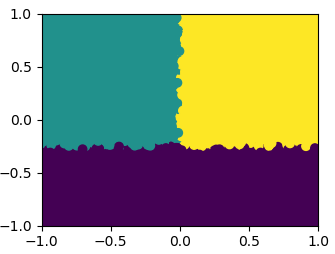
\includegraphics[scale=0.6]{assets/target}
  \caption{Objectif}
\end{figure}

On construit un réseau de neurones ayant les couches suivantes:
\begin{enumerate}
  \item couche d'entrée de 2 neurones;
  \item couche \textsc{relu} à 4 sorties;
  \item couche \textsc{softmax} à 3 sorties.
\end{enumerate}

\begin{figure}[h]
  \centering
  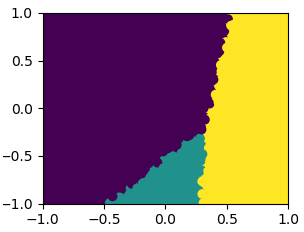
\includegraphics[scale=0.7]{assets/random}
  \caption{Réseau initialisés avec une $\mathcal{N}(0, 1)$}
\end{figure}

On entraîne le réseau en utilisant une descente de gradient stochastique:
\begin{itemize}
  \item 10000 échantillons d'entraînement;
  \item 20 \textit{epoch};
  \item \textit{batch} de taille 500;
  \item taux d'apprentissage $\eta = 1$.
\end{itemize}

\begin{figure}[h]
  \centering
  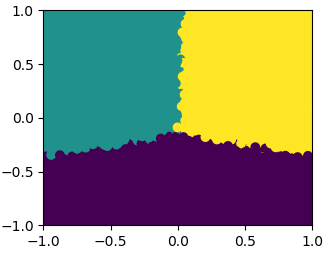
\includegraphics[scale=0.6]{assets/trained}
  \caption{Réseau entraîné.}
\end{figure}

On obtient un taux de classification correcte de l'ordre de 96\%.


\end{document}
